%!TEX root=rapport.tex

\section{Interprétation des résultats obtenus}

\subsection{Résultats finaux}

Expliquer le principe du dotmatch , avec "projection sur l'axe x"

Interprétaiton des résultats -> ça couvre globalement bien sauf pe pour la 2 + dire qu'il y en a qui sont trop longs! (ou trop court)

\noindent\textbf{Cible 1}





\begin{figure}[!ht]
	\begin{minipage}[r]{.46\linewidth}
		\begin{center}
		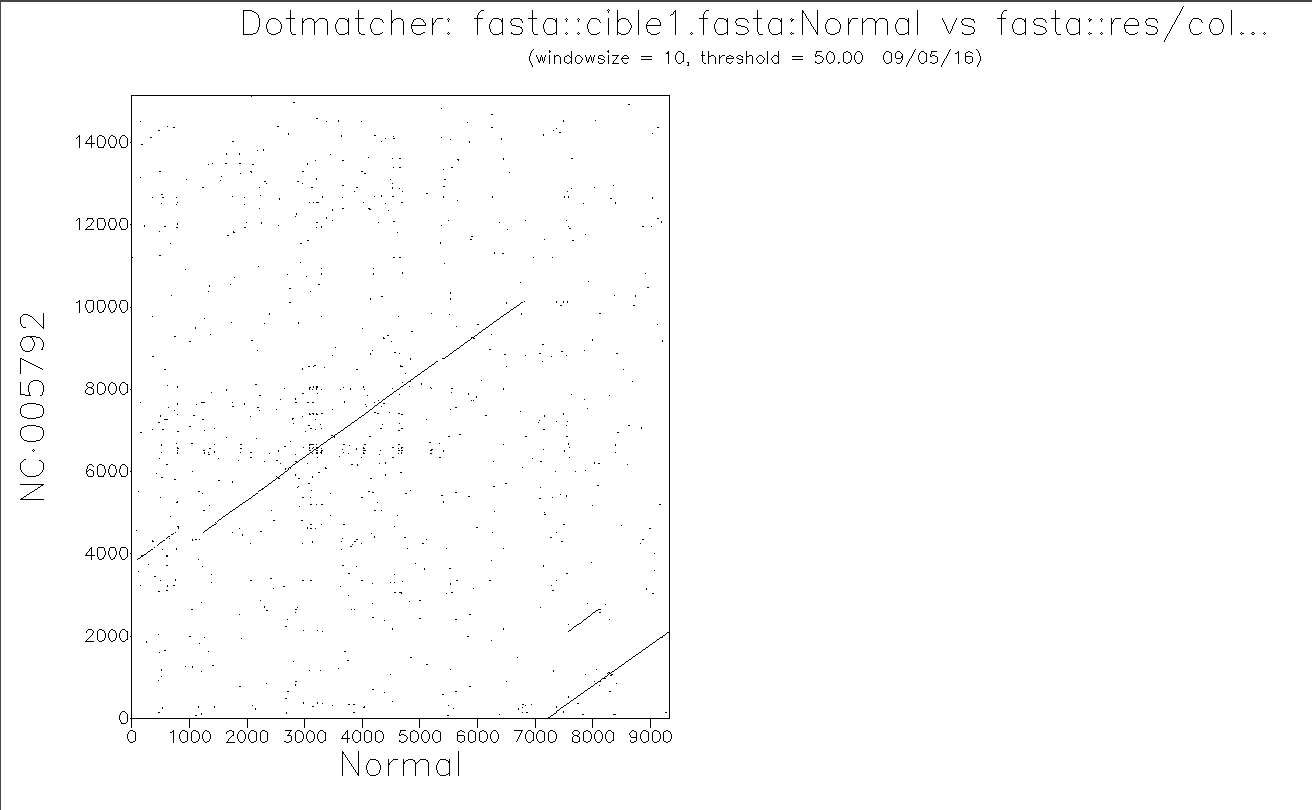
\includegraphics[scale= 0.4]{../res/cible1.png}
		Résultat de la collection 1
	\end{center}
\end{minipage} \hfill
\begin{minipage}[c]{.46 \linewidth}
	\begin{center}
			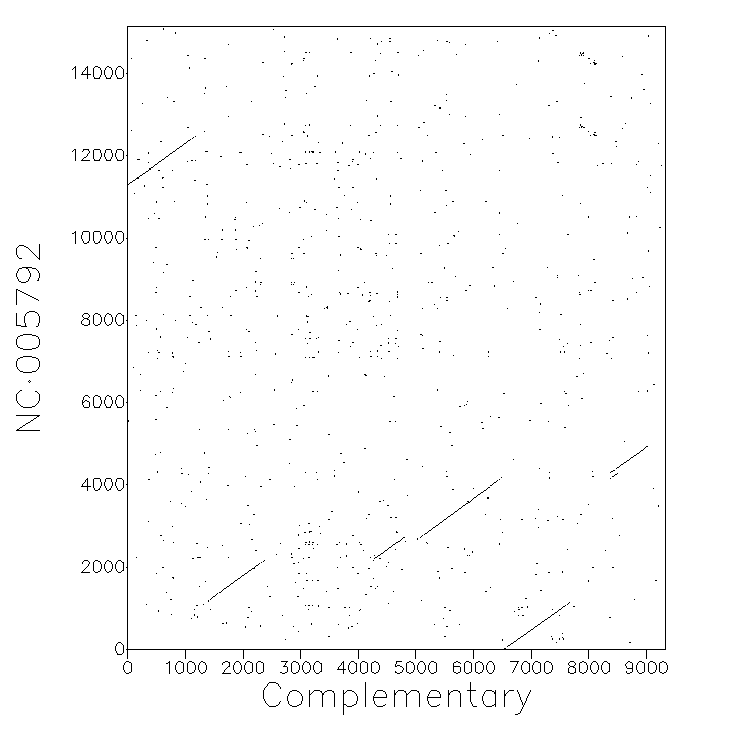
\includegraphics[scale= 0.4]{../res/cible1-ic.png}
			Résultat de la collection 1, complémenté et inversé
		\end{center}
	\end{minipage}
	\caption{Résultat de la collection 1}
\end{figure}

\FloatBarrier


\noindent\textbf{Cible 2}


\begin{figure}[!ht]
	\begin{minipage}[r]{.46\linewidth}
		\begin{center}
		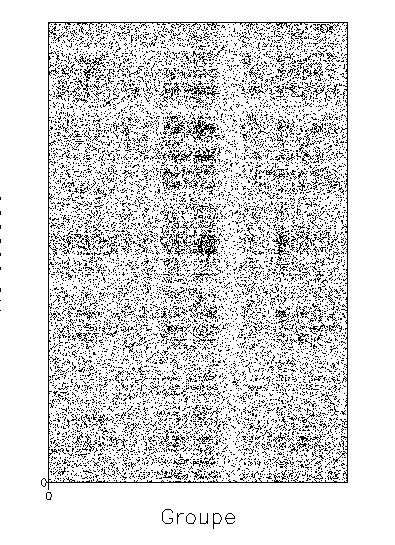
\includegraphics[scale= 0.4]{../res/cible2.png}
		Résultat de la collection 2
	\end{center}
\end{minipage} \hfill
\begin{minipage}[c]{.46 \linewidth}
	\begin{center}
			%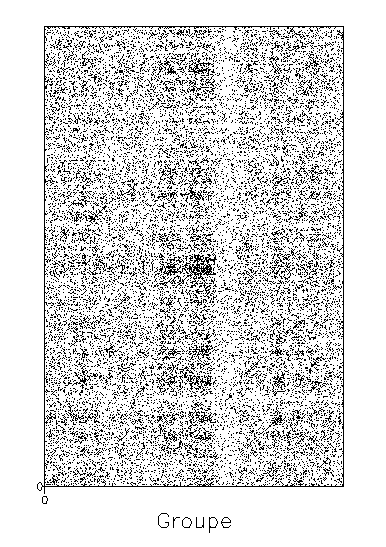
\includegraphics[scale= 0.4]{../res/cible2-ic.png}
			Résultat de la collection 2, complémenté et inversé
		\end{center}
	\end{minipage}
	\caption{Résultat de la collection 2}
\end{figure}

\FloatBarrier


\noindent\textbf{Cible 4}

\begin{figure}[!ht]
	\begin{minipage}[r]{.46\linewidth}
		\begin{center}
		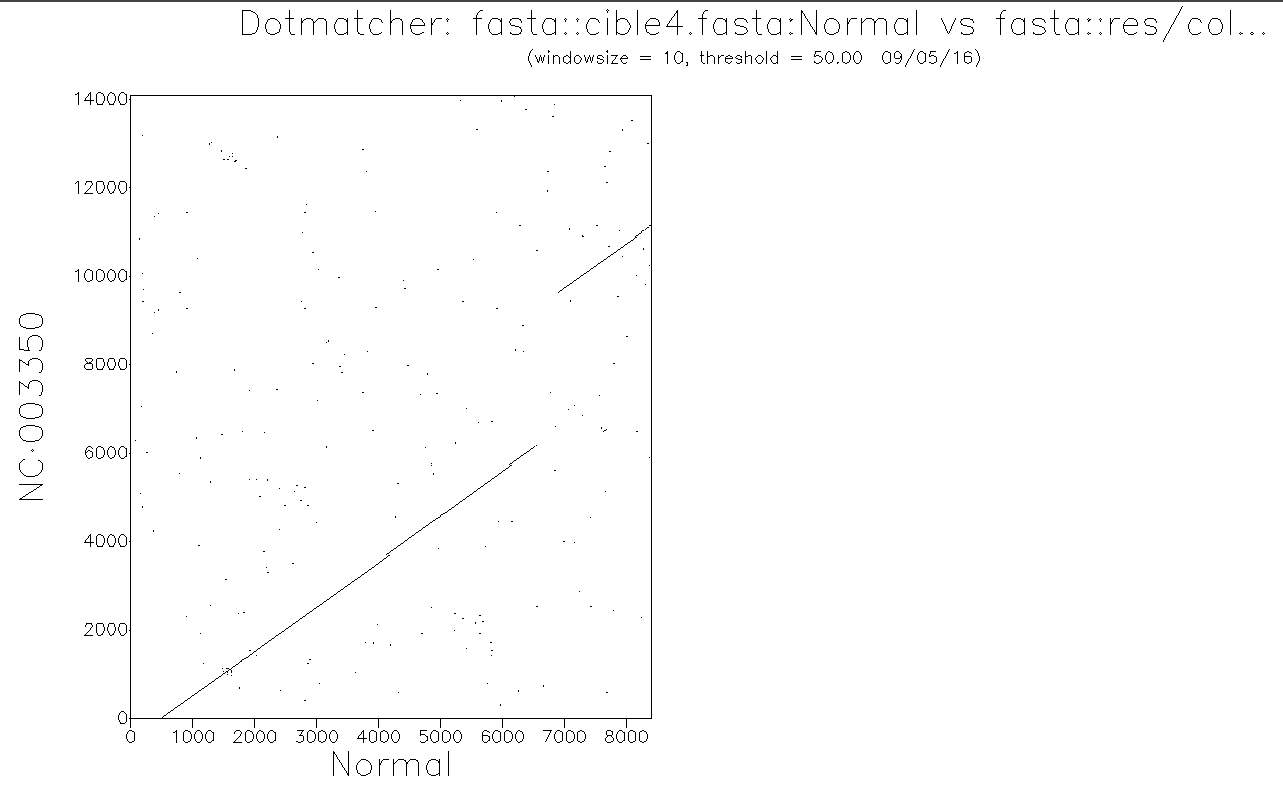
\includegraphics[scale= 0.4]{../res/cible4.png}
		Résultat de la collection 4
	\end{center}
\end{minipage} \hfill
\begin{minipage}[c]{.46 \linewidth}
	\begin{center}
			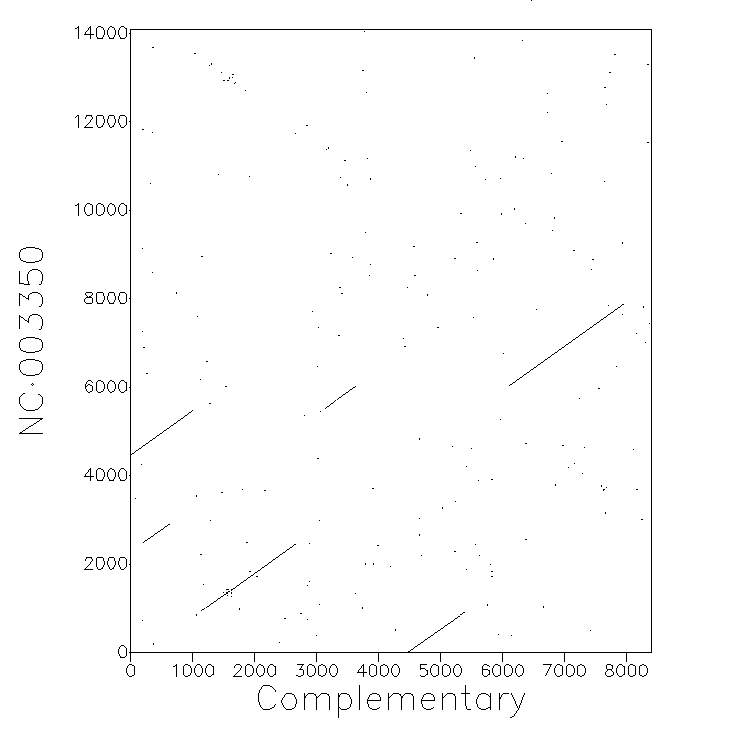
\includegraphics[scale= 0.4]{../res/cible4-ic.png}
			Résultat de la collection 4, complémenté et inversé
		\end{center}
	\end{minipage}
	\caption{Résultat de la collection 4}
\end{figure}

\FloatBarrier


\noindent\textbf{Cible 5}

\begin{figure}[!ht]
	\begin{minipage}[r]{.46\linewidth}
		\begin{center}
		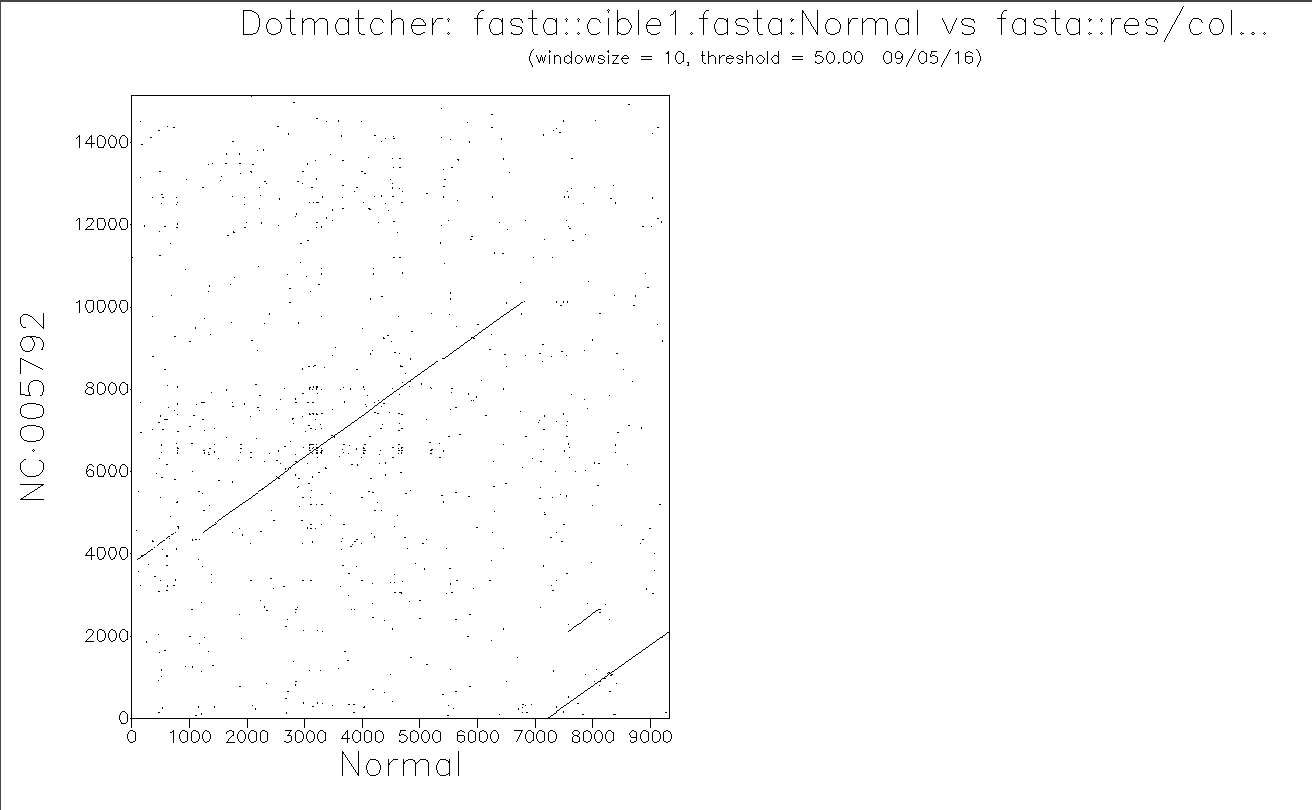
\includegraphics[scale= 0.4]{../res/cible1.png}
		Résultat de la collection 5
	\end{center}
\end{minipage} \hfill
\begin{minipage}[c]{.46 \linewidth}
	\begin{center}
			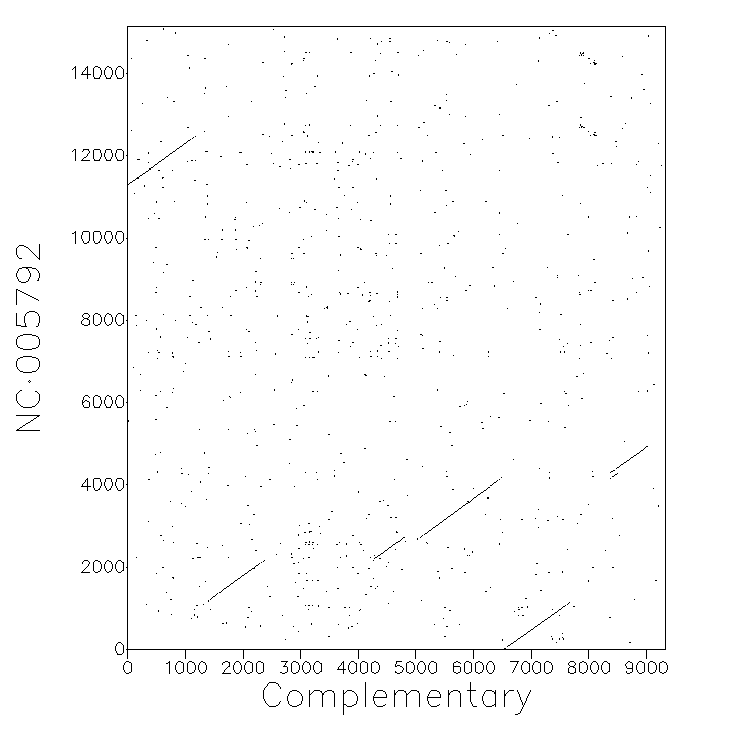
\includegraphics[scale= 0.4]{../res/cible1-ic.png}
			Résultat de la collection 5, complémenté et inversé
		\end{center}
	\end{minipage}
	\caption{Résultat de la collection 5}
\end{figure}



\FloatBarrier

\subsection{Autres implémentations}

Nous avons également tenté de changer l'implémentation du Greedy en changeant
le comparateur d'arcs, en prévilégiant les nombres de gaps finaux et initiaux
dans l'alignement semi-global des séquences ou en propageant les gaps à la fin.

Par exemple, lorsque deux arcs ont un même score, nous avons tenté de
privilégier les arcs qui ont une plus longue sous-séquence commune, c'est-à-dire
sans compter les gaps finaux et initiaux. Cette méthode ne nous a pas donné de
mauvais résultats mais ils étaient moins bons.

Dans le code soumis, nous avons prévilégié, lors de l'alignement semi-global,
l'alignement avec le moins de gaps finaux et initiaux, c'est-à-dire en
prenant le dernier maximum pour la dernière colonne et la dernière ligne. Nous
avons tenté de prendre le premier maximum pour chacun d'entre eux, mais cela n'a
pas donné de meilleurs résultats non plus.

%Explication de la propagations des gaps à la fin.
